\documentclass[12pt,utf8]{beamer}

% Gute Einführung zu LaTeX-Beamer: http://www2.informatik.hu-berlin.de/~mischulz/beamer.html

%-----PARAMETERS-----

%Wichtige Standard Pakete!
%\usepackage[german]{babel}
\usepackage{ngerman}
\usepackage{xcolor}
\usepackage{graphicx}
\usepackage{tikz}

%Für den Header notwendig!
%\usepackage[percent]{overpic}


\usepackage{hyperref} % für korrekte Links

%Einbinden des Themes
%
% TU
% A Beamer theme with the colors of the TU Dortmund.
%
% Author: Kevin Dungs (https://github.com/kdungs)
% Version: 0.2 2013-05-15
%

%\usepackage{fontspec}
 %   \setmainfont[Ligatures=TeX]{Tex Gyre Adventor}
\usepackage{xcolor}


% Colors
\definecolor{TUgreen}{HTML}{649600}
\definecolor{TUgreenLighter}{HTML}{A5CB5B}
\definecolor{TUgreenDarker}{HTML}{54711C}
\definecolor{TUalert}{HTML}{A10000}
\definecolor{TUalertLighter}{HTML}{D03434}
\definecolor{TUexample}{HTML}{006496}
\definecolor{TUexampleLighter}{HTML}{8735B5}
\definecolor{PeP}{HTML}{565656}
\definecolor{ltgrey}{HTML}{CCCCCC}

% Titlepage
%  Title
\setbeamerfont{title}{size=\Huge}
\setbeamercolor{title}{fg=white, bg=TUgreen}
%  Subtitle
\setbeamerfont{subtitle}{size=\large}
%  Author
%\setbeamerfont{author}{size=\large}
%  Institute
\setbeamerfont{institute}{series=\bfseries, size=\small}
\setbeamercolor{institute}{fg=PeP}

% Frametitle
\setbeamerfont{frametitle}{size=\Huge}
\setbeamercolor{frametitle}{fg=white, bg=TUgreen}

% Framesubtitle
\setbeamerfont{framesubtitle}{size=\Large}
\setbeamercolor{framesubtitle}{fg=white, bg=TUgreenDarker}

% Structure
\setbeamerfont{structure}{size=\Large}
\setbeamercolor{structure}{fg=TUgreen}

% Blocks
\setbeamertemplate{blocks}[square]
\setbeamerfont{block title}{}
\setbeamercolor{block title}{fg=TUgreen, bg=white}
\setbeamercolor{block title alerted}{use=alerted text,fg=TUalert, bg=white}
\setbeamercolor{block title example}{use=example text,fg=TUexample, bg=white}

% Items
\setbeamertemplate{items}[circle]

% Other
\setbeamertemplate{navigation symbols}{} %no nav symbols

% Customizations


\setbeamertemplate{frametitle}
{
  \ifx\insertframesubtitle\empty
  	\vspace*{.5em}
  	\begin{beamercolorbox}[wd=.92\paperwidth, ht=1em, dp=.4em, leftskip=.04em, left]{frametitle}
  		\hspace{.25em}\usebeamercolor{frametitle}\usebeamerfont{frametitle}\insertframetitle 
  	\end{beamercolorbox}
  \else
    \vspace*{.5em}
    \begin{beamercolorbox}[wd=.92\paperwidth, ht=1em, dp=.4em, leftskip=.04em, left]{frametitle}
    	\hspace{.25em}\usebeamercolor{frametitle}\usebeamerfont{frametitle}\insertframetitle 
    \end{beamercolorbox}
    \begin{beamercolorbox}[wd=.92\paperwidth, ht=.7em, dp=.3em, leftskip=.04em, left]{framesubtitle}
    	\hspace{.25em}\usebeamercolor{framesubtitle}\usebeamerfont{framesubtitle}\insertframesubtitle
    \end{beamercolorbox}   
  \fi
}

\defbeamertemplate*{footline}{TU}
{
    \leavevmode%
    \begin{beamercolorbox}[wd=.1\paperwidth, ht=1.8em, dp=1em, left, leftskip=1em]{}%
        \textbf{\insertshorttitle}
    \end{beamercolorbox}%
    \begin{beamercolorbox}[wd=.8\paperwidth, ht=1.8em, dp=1em, center, rightskip=4em]{}%
        \insertshortauthor\quad(\insertshortinstitute)%
    \end{beamercolorbox}%
    \begin{beamercolorbox}[wd=.1\paperwidth, ht=1.8em, dp=1em, right, rightskip=1em]{}%
        \insertframenumber{} / \inserttotalframenumber%
    \end{beamercolorbox}%
}

%Standard Angaben
\title{Die FOSS-AG}
\subtitle{Was machen die eigentlich?}

\author[J.-M. Lenk, C. Parnitzke, J. Schneider]{Jan-Marius Lenk, Christoph Parnitzke, Josef Schneider}
\institute[FOSS AG]{Free and Open Source Software AG\\ Fakultät für Informatik}

\date{\today}

%-----IMPLEMENTATION-----

\begin{document}

\begin{frame}
	\titlepage
\end{frame}

\section{Einleitung}

\begin{frame}{Inhaltsverzeichnis}
	\tableofcontents[currentsection, hideallsubsections]
\end{frame}

\begin{frame}{Wer sind die...}{...und was wollen die?}
	Die \textbf{F}ree and \textbf{O}pen \textbf{S}ource \textbf{S}oftware \textbf{AG} stellt sich vor... 
\end{frame}

\begin{frame}
\frametitle{Was machen wir?}
\begin{itemize}
	\item Vortragsreihen
	\item Installationspartys
	\item Orientierungsphase Informatik TU Dortmund
	\item Zusammenarbeit mit den lokalen Hackspaces
	\item Raspberry Pi Projekte an Schulen
	\item Linux-HelpDesk
\end{itemize}
\end{frame}

\begin{frame}
	\frametitle{Wo findet man uns?}
	\begin{itemize}
		\item foss-ag.de
		\item Social Media: Telegram, Riot, Twitter
		\item wöchentliche Treffen an der TU Dortmund\\(siehe Homepage)
	\end{itemize}
\end{frame}

\begin{frame}
\frametitle{Wir haben für euch geplant:}
\begin{figure}

\includegraphics[scale=0.1]{resources/linuxcalm.png}
\end{figure}
	\begin{itemize}
		\item Software \& Desktops unter Linux + offene Diskussionsrunde
		\item Linux - Installparty
	\end{itemize}
\end{frame}

\begin{frame}
\frametitle{Wir haben für euch geplant:}
	\begin{itemize}
		\item Dateisystem
		\item Einführung in die Kommandozeile
		\item SSH - Tipps und Tricks
		\item Python-Scripting
	\end{itemize}
\end{frame}

\begin{frame}
\frametitle{Wir haben für euch geplant:}
\begin{itemize}
	\item Advanced-Vortrag Kommandozeile
	\item Free my Android
	\item Backups mit Borg
\end{itemize}
\end{frame}

%\begin{frame}[<-+>]{Wer sind die...}{...und was wollen die?}
%	\textquotedblleft Unser Ziel ist es freie, quelloffene oder gemeinnützige Projekte technisch zu unterstützen.\textquotedblright \\
%	Wir unterstützen ausserdem auch die Menschen selbst. Zum Beispiel euch! \\
%	Aber wie können wir euch am Besten helfen? Indem wir unser Wissen mit euch teilen. \\
%	Daher wollen wir euch jetzt unser Verständnis von FOSS und die Liebe zu Linux und freier Software euch nahe bringen.
%\end{frame}

%//end of section "Einleitung"

\section{Theorie}

\begin{frame}{Inhaltsverzeichnis}
	\tableofcontents[currentsection, hideallsubsections]
\end{frame}



%\begin{frame}
%\frametitle{Wer entwickelt Linux?}
%\begin{figure}
%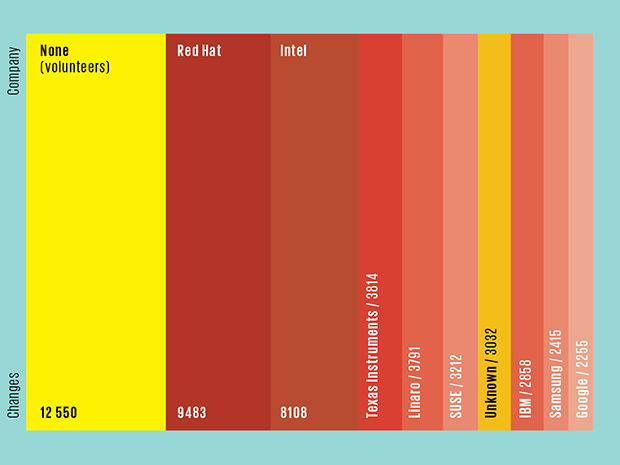
\includegraphics[scale=0.4]{resources/linuxdev.jpg}
%\end{figure}
%http://www.extremetech.com/wp-content/uploads/2014/02/02DataFlowBills3-1390852937757.jpg
%\end{frame}

\begin{frame}
\frametitle{Free vs. OS vs. Kostenlos}
\begin{figure}

\includegraphics[scale=0.5]{resources/open_swiss_knife.png}
\end{figure}
%Open-Source beschränkt sich nicht nur auf Software
\begin{itemize}
	\item Open-Source == Freies Wissen
	%open source ist denkweise...Wissen soll für alle frei sein
	\item Open-Source Software == Software mit frei zugänglichem Quellcode
	\item Free Software:
	\begin{itemize}
		\item 1. Freiheit der Kontrolle über Software
		%totale Kontrolle über alle Aspekte der Software: Analyse und Änderung. Quellcode muss nicht erhalten werden
		\item 2. Soziale Freiheit der Kolaboration
		%Verbreitung des Quellcodes. Auch kommerzielle Tätigkeiten dürfen angeboten werden
	\end{itemize}
	\item Kostenlose Software (Freeware) == Programmierer verzichtet auf Nutzungsvergütung
	%Freeware Nutzung wird eingeräumt, Änderung allerdings nicht
	%https://de.wikipedia.org/wiki/Datei:121212_2_OpenSwissKnife.png
\end{itemize}

%\footnote{https://de.wikipedia.org/w/index.php?search=kostenlose+Software&title=Spezial$%$3ASuche&fulltext=Volltext}
\end{frame}

\begin{frame}
	\Huge Warum ist Open-Source cool?
\end{frame}

\begin{frame}
	\centering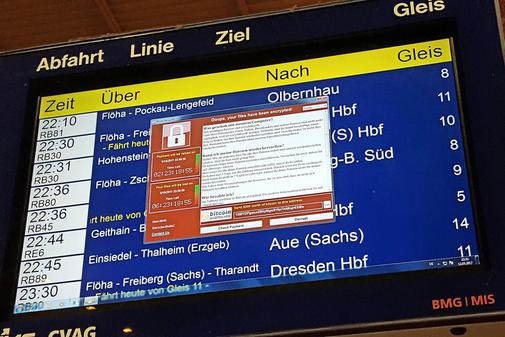
\includegraphics[scale=1.7]{resources/wannacrydb.jpg}
\end{frame}

\begin{frame}
\frametitle{Warum ist Open-Source cool?}
\begin{figure}

\includegraphics[scale=0.4]{resources/att.jpg}
\end{figure}
\begin{itemize}
	\item Fehlerbehebung durch Community
	%Bug Hunting
	\item Schwachstellen und potentielle Angriffsstellen werden erkannt
	%Zero-Date exploits, Backdoors
	\item Kontrolle bzgl. unerwünschter Nebenfunktionen
	%Funktionen zur Überwachung oder zur Erstellung von Hintertüren
\end{itemize}
%\footnote{https://www.bing.com/images/search?q=open+source+meme&view=detailv2&&id=3CEEA01A1F60BB879267791D1040EEB7081F26B2&selectedIndex=101&ccid=0j9v2qqY&simid=607986818429160812&thid=OIP.ee0ac8a908656d52412286fa1abe398f&ajaxhis+t=0}
\end{frame}


\begin{frame}
\frametitle{Linux - Motivation}

\begin{tabular}{cl}
	\begin{tabular}{c}
		
\includegraphics[scale=0.35]{resources/grandmaLinux.jpg}
	\end{tabular}
	& \begin{tabular}{l}
		\parbox{0.5\textwidth}{\begin{itemize}
	\item Linux ist überall
	\begin{itemize}
		\item Server
		\item Arbeitsplatz
		\item Smartphone
	\end{itemize}
	\item Linux ist einfach
	\begin{itemize}
		\item Simple Oberfläche
		\item Stabiles System
		\item Gleiche Funktionalität wie andere Systeme
	\end{itemize}
	%https://2.bp.blogspot.com/_UqUwVPikChs/TFq5scy4dVI/AAAAAAAAOiM/tDuYjZGTSgY/s1600/GrandmaLinux.jpg
\end{itemize}}
	\end{tabular}

\end{tabular}
\end{frame}

\begin{frame}
\frametitle{Was ist Linux?}
\begin{figure}

\includegraphics[scale=0.17]{resources/tux.png}
\end{figure}
\begin{itemize}
	\item Free and Open-Source Mehrbenutzer-Betriebssystem
	\item Basiert auf dem Linux-Kernel
	%von Linus Torvalds für x86 architecture entwickelt
	%Kernel ist Schnittstelle zwischen Software und Hardware
	%Geschrieben in C
	\item Projekt wird unterstützt von Unternehmen, Non-Profit-Organisationen und vielen Freiwilligen
	\item Linux-Distro fasst Kernel und unterschiedliche Software zusammen
	%https://upload.wikimedia.org/wikipedia/commons/a/af/Tux.png
\end{itemize}
\end{frame}

%\begin{frame}
%\frametitle{Was bietet Linux?}
%\begin{figure}
%
\includegraphics[scale=0.33]{resources/kitteh.jpg}
%\end{figure}
%\begin{itemize}
%	\item Sicher
%	\item Modifizierbar
%	\item Kostenlos
%\end{itemize}
%\footnote{http://danlynch.org/wp-content/uploads/2009/04/funny-pictures-your-kitten-uses-linux.jpg}
%\end{frame}

%\begin{frame}
%\frametitle{Was macht Linux sicher?}
%\begin{figure}
%
\includegraphics[scale=0.3]{resources/infosec.jpg}
%\end{figure}
%\begin{itemize}
%	\item Tausende von Entwicklern prüfen den Code auf Fehler
%	\item Große Firmen haben Teams von ca. 10-30 Leuten 
%	\begin{itemize}
%		\item Meist nicht genug Geld und Zeit für Prüfung geplant
%		\item Prüfung erfolgt meist generisch
%	\end{itemize}
%	\item Vertrauen der Entwickler untereinander
%	\item Denkweise der Entwickler ist anders
%\end{itemize}
%http://www.valiantsolutions.com/images/infosec.jpg
%\end{frame}



%\\end of section "Theorie"

\section{Praxis}

\begin{frame}{Inhaltsverzeichnis}
	\tableofcontents[currentsection, hideallsubsections]
\end{frame}



\subsection{Distros}
\begin{frame}
\frametitle{Was ist eine Dist.?}
Betrieben von Community/Firmen.
Kümmern sich um: 
\begin{itemize}
 \item Pakete
 \item Änderungen/Patches
 \item Hilfe/Support
\end{itemize}
 
\end{frame}

\begin{frame}
 \frametitle{Vorkommen}

 
 \begin{itemize}
  \item Raspian/Kodi/..
  \item Android/Sailfish
  \item Alpine/TinyCore/CoreOS
  \item viele embedded Geräte mit speziell angepasstem Linux
 (wie Router, Steuergeräte, Mediengeräte)
 \end{itemize}

\end{frame}



\begin{frame}
\frametitle{Bsp. Distros}
\begin{itemize}%[<+->]
\item Debian
\item Ubuntu
\item Mint
\item Arch
\item openSuse
\item RHEL/Fedora/CentOS 
\item gentoo
\item Puppy/Knoppix 

\item Kali 

\end{itemize}
\end{frame}

\subsection{Oberflächen}
\begin{frame}
\frametitle{Oberflächen}

\begin{multicols}{2}
\onslide<1->{\begin{figure}
 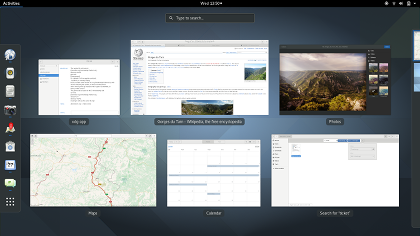
\includegraphics[width=0.45\textwidth]{resources/window-selection.png}
%\footnote{https://www.gnome.org/wp-content/uploads/2016/03/window-selection-3.20-420x236.png}
 \end{figure}
}
\onslide<2->{

\begin{figure}
 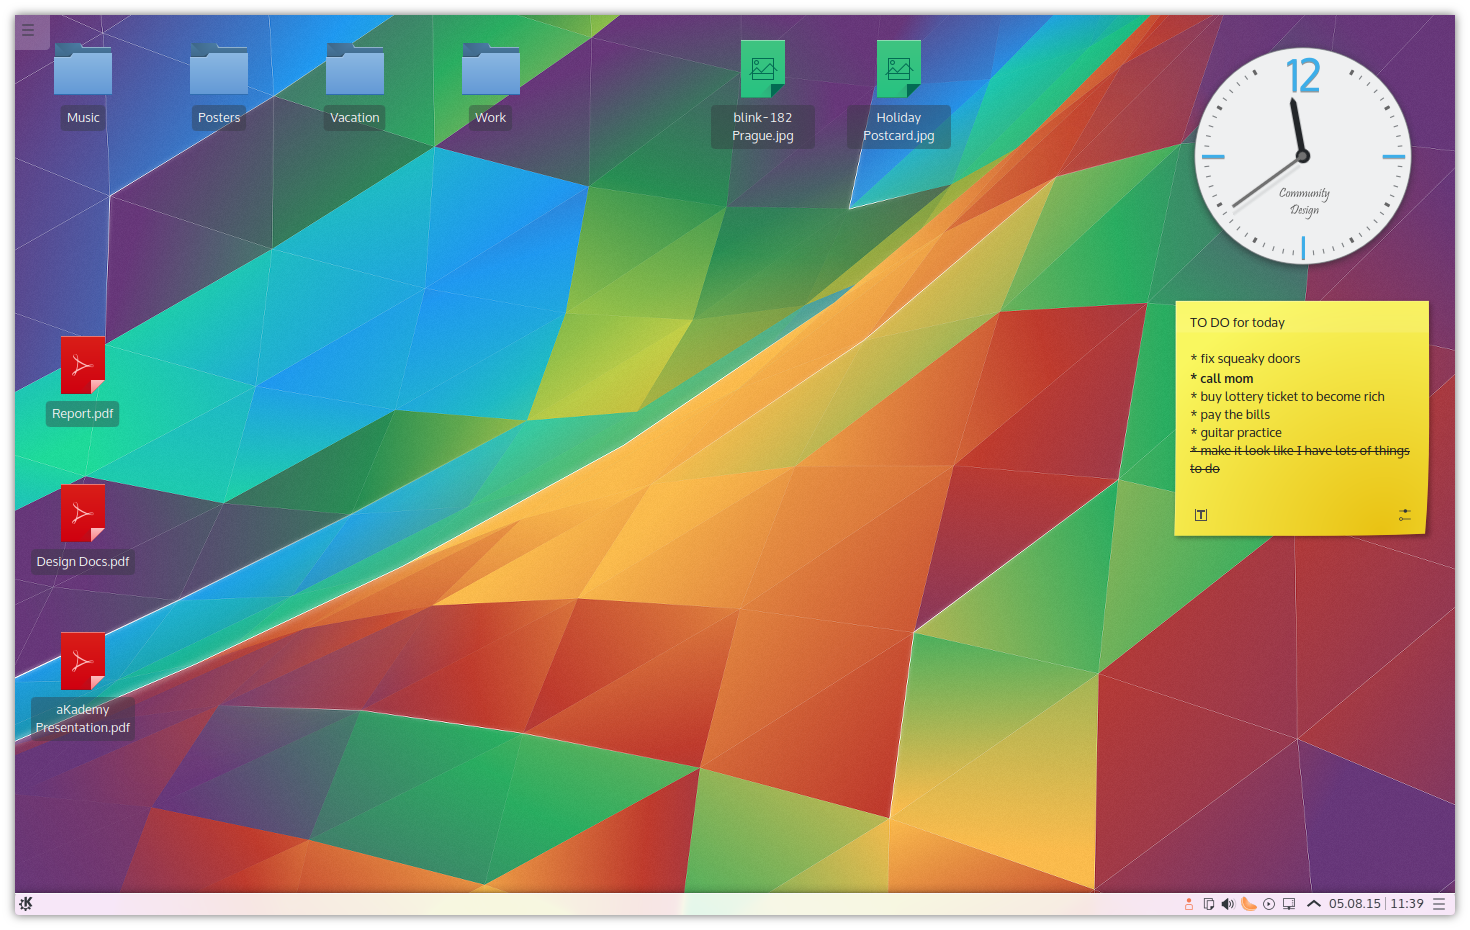
\includegraphics[width=0.45\textwidth]{resources/general-desktop.png}
\end{figure}
%\footnote{https://www.kde.org/workspaces/plasmadesktop/screenshots/general-desktop.png}
}


\only<1>{Gnome}
\only<2>{KDE: Plasma}
\only<3>{Unity (Ubuntu)}
\onslide<4>{\begin{figure}
  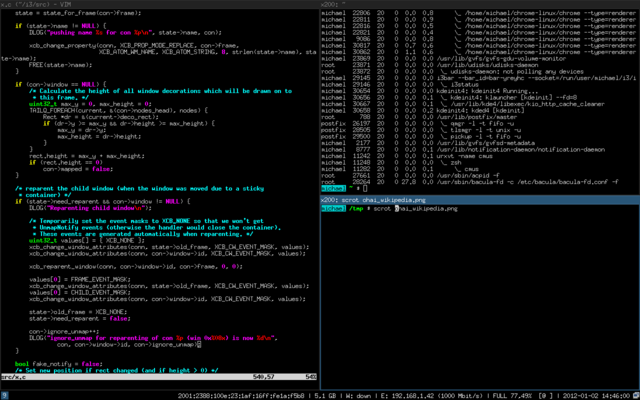
\includegraphics[width=0.45\textwidth]{resources/I3_window_manager_screenshot.png} %Nammensnennung!!
  %footnote{https://de.wikipedia.org/wiki/I3_(Fenstermanager)#/media/File:I3_window_manager_screenshot.png}
  \end{figure}
  
  \onslide<3->{\begin{figure}
  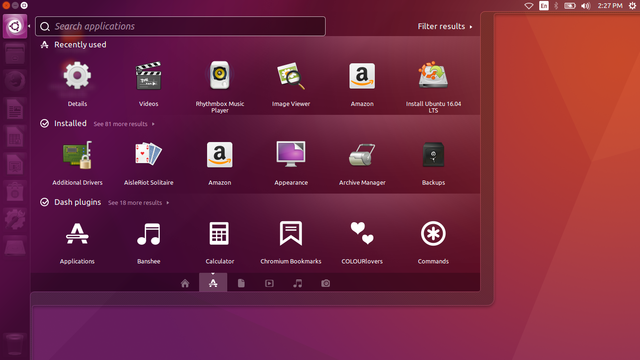
\includegraphics[width=0.45\textwidth]{resources/App_Lens_on_Ubuntu_16.png}
 %\footnote{https://en.wikipedia.org/wiki/Unity_(user_interface)#/media/File:App_Lens_on_Ubuntu_16.04LTS.png}
\end{figure}}
}

%\begin{itemize}
%\item Gnome3
%\item KDE
%\item mate
%\item Konsole
%\end{itemize}

\end{multicols}

\end{frame}


\subsection{Programme}
\begin{frame}[allowframebreaks]
 \frametitle{Programme}
 %\begin{tabular}{lp{5cm}}
 %Kategorie& Software \\ \hline
 
\hspace{1cm}

\begin{description}[style=nextline]

 \item [Browser] {\bf Firefox}, Chromium, Vivaldi, Opera, Tor

 \item [Office] {\bf LibreOffice}, Kile (\LaTeX), \TeX maker

 \item [Email Clients] {\bf Thunderbird}, Icedove, Evolution 

 \item [Messenger] Pidgin, Empathy, HexChat, Telegram

 \item [VoIP] Mumble, Ring, Tox

 \item [Synchronisation] Nextcloud, Owncloud, Seafile
\pagebreak 
 \item [IDEs] {\bf Eclipse}, IntelliJ, NetBeans, Atom, VI(M)

 \item [Medien]{\bf VLC}, Audacity, Rythmbox, Totem

 \item [Grafik] {\bf GIMP}, Blender,  Inkscape

 \item [System] {\bf Wireshark}, GParted, Boabab, Filezilla

 \item [Torrents] Transmission 

 \item [alles] DAS TERMINAL 

\end{description}
 \end{frame}






%\\end of section "Praxis"

\section{Termine}

\begin{frame}{Creative-Commons Musik}
	\scriptsize {
		\begin{itemize}
			\item Broke For Free - Layers (CC BY-NC 3.0)
			\item Broke For Free - SomethingEP (CC BY-NC 3.0 / CC BY 3.0 US)
			\item Asthmatic Astronaut - Exposing All Emotions (CC BY-NC-SA 3.0 US)
			\item Chris Zabriskie - Reappear (CC BY 4.0)
			\item Drake Stafford - SUNDAY (CC BY 4.0)
			\item Ghosts - Judge EP (CC BY-NC-SA 3.0)
			\item LASERS - LASERS EP (CC BY-NC-SA 3.0)
			\item Little Glass Men - Simplify (CC BY 4.0)
			\item Little Glass Men - The Age of Insignificance (CC BY 4.0)
			\item Pierlo - Saturday Night Sleeper (CC BY-NC-SA 2.5 IT)
			\item Tours - Enthusiast (CC BY 3.0)
		\end{itemize}
	}
\end{frame}

\begin{frame}{Creative-Commons Lizenzen}
	\scriptsize {
		\begin{itemize}
			\item CC BY-NC-SA 2.5 IT\\ https://creativecommons.org/licenses/by-nc-sa/2.5/it/legalcode
			
			\item CC BY-NC 3.0\\
			https://creativecommons.org/licenses/by-nc/3.0/legalcode
			
			\item CC BY 3.0\\
			https://creativecommons.org/licenses/by/3.0/legalcode
			
			\item CC BY 3.0 US\\
			https://creativecommons.org/licenses/by/3.0/us/legalcode
			
			\item CC BY-NC-SA 3.0\\
			https://creativecommons.org/licenses/by-nc-sa/3.0/legalcode
			
			\item CC BY-NC-SA 3.0 US\\
			https://creativecommons.org/licenses/by-nc-sa/3.0/us/legalcode
			
			\item CC BY 4.0\\
			https://creativecommons.org/licenses/by/4.0/legalcode
	\end{itemize}
	}
\end{frame}

\begin{frame}{Image-sources - 1}
	Dies sind die Quellen der Bilder, die für die Präsentation benutzt wurden, sortiert nach ihrem Auftreten.
	\begin{itemize}
		\item [1] 2.bp.blogspot.com/\textunderscore UqUwVPikChs/TFq5scy4dVI/AAAAAAAAOiM/tDuYjZGTSgY/s1600/GrandmaLinux.jpg
		\item [2] upload.wikimedia.org/wikipedia/commons/a/af/Tux.png
		\item [3] www.extremetech.com/wp-content/uploads/2014/02/02DataFlowBills3-1390852937757.jpg
		
		\item [4] upload.wikimedia.org/wikipedia/commons/c/c7/121212\textunderscore 2\textunderscore OpenSwissKnife.png
		\item [5] www.bizcoder.com/Media/Bizcoder/Windows-Live-Writer/715c931eba8c\textunderscore 7522/AllTheThings\textunderscore 2.jpg
	\end{itemize}
\end{frame}

\begin{frame}{Image-sources - 2}
	\begin{itemize}
		\item [6] danlynch.org/wp-content/uploads/2009/04/funny-pictures-your-kitten-uses-linux.jpg
		\item [7] www.valiantsolutions.com/images/infosec.jpg
		\item [8] https://pixabay.com/en/garbage-electronics-trash-rubbish-296550/
		\item [9] By gg3po, Iwan Gabovitch - Tux Flat SVG, based on File:NewTux.svg by gg3po which is based on File:Tux.png byLarry Ewing, GPL, \url{https://commons.wikimedia.org/w/index.php?curid=48629023}
		\item [9] David Swanson - Laptop icon from The Noun Project. \url{https://commons.wikimedia.org/wiki/File:Noun_project_143222.svg}
		\item [10] PAZ Online - WannaCry Deutsche Bahn.
		\url{http://www.paz-online.de/var/storage/images/rnd/wirtschaft/uebersicht/wanna-cry-ist-weckruf-fuer-viele-firmen/581383990-1-ger-DE/Wanna-Cry-ist-Weckruf-fuer-viele-Firmen_pdaArticleWide.jpg}
	\end{itemize}
\end{frame}


%\\end of section "Schluß"



\end{document}
